\documentclass[a4paper]{report}

%\synctex=1
%\usepackage[T1]{fontenc} %better input encoding for glyphs and hyphenation 
\usepackage[utf8]{inputenc} %input encoding for most general keyboards (better)
\usepackage{lmodern}
\usepackage[english]{babel} 

\usepackage{url}
\usepackage{amsmath}
\usepackage{amssymb}
\usepackage{amsfonts}
\usepackage{amsthm}
\usepackage{xfrac}
\usepackage{xcolor}
\usepackage[pdftex]{hyperref}
\hypersetup{
    colorlinks,
    linkcolor={blue!60!black},
    citecolor={blue!50!black},
    urlcolor={blue!80!black}
}
\usepackage{multirow}
\usepackage{booktabs}
\usepackage{dcolumn}
\usepackage{anysize}
%\marginsize{1.4in}{1.4in}{1in}{1in}
\usepackage[format=hang,labelfont=bf,up,textfont=it,up]{caption}
\setlength{\captionmargin}{20pt}


\usepackage{tikz}
\usetikzlibrary{mindmap,trees}
\usetikzlibrary{positioning,shadows,shapes,arrows}
\pgfdeclarelayer{background}
\pgfsetlayers{background,main}
\usepackage{soul} 

\newtheorem{defi}{Definition}
\newtheorem{teo}{Theorem}
\newtheorem{axi}{Principle}





\begin{document}


\begin{titlepage}
\begin{center}
\end{center}
\vspace{3cm}
\begin{flushleft}
\end{flushleft}
\hrule height 1.2pt
\vspace{2cm}
\begin{center}
\textbf{\Huge  Aerospace Course Notes \\[5mm] Classical ThermoMechanics}\\[3cm]			
\hrule
\vspace{1.0cm}
\large \today
\end{center}
\hrule height 1.2pt
\vfill
\begin{flushleft}
\footnotesize 
Instituto Superior de T\'ecnico - Lisboa - Portugal \\
\end{flushleft}
\end{titlepage}


\tableofcontents

\chapter{Fundamental Laws}
\newpage
\section{Maxwell's Equations}



\chapter{Fundamental Circuit Laws}
\newpage
\section{Kirchoff Voltagem Law (KVL)}
\subsection{Voltage Signals}
\section{Kirchoff Current Law (KCL)}
\subsection{Current Signals}






\chapter{Circuit Elements}

\section{Voltage Sources}

\section{Current Sources}

\section{Resistance}
So resistance is a fundamental property of electricmagnetic property that can it self be determined from the Maxwell equation. However the macroscopic Ohm law is the one more often used in electric and electronic circuits. So the impedance of a resistance is give by \ref{zresistance}.

\begin{equation} \label{zresistance}
Z_R=R=\frac{v}{i}
\end{equation}

The symbol for a resistor, i.e. a element that has only resistance, is shown in figure \ref{fig_res}.


\begin{figure}

\end{figure}


\section{Capacitance}

\section{Inductance}


\section{Diode}
So a diode is many times considered has a nonlinear resistance  witch the current varies according to \ref{idiode} . Here we also define the diode operator $\delta(v)$ which will be very usfull when analysing the Bipolar Junction Transistor (BJT).

\begin{figure}[H]
\begin{center}
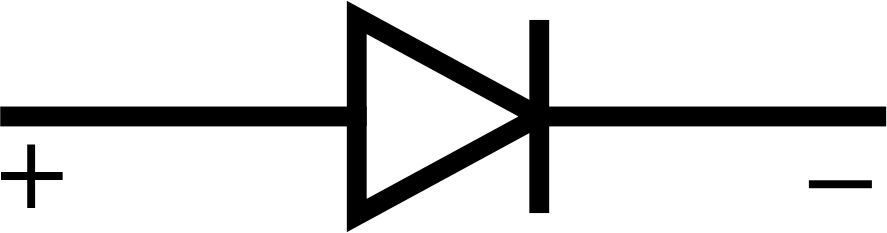
\includegraphics[scale=.12]{diode_symb.png}
\end{center}
\end{figure}

\begin{equation} \label{idiode}
i_D=I_{S}(e^{\frac{v_D}{\eta V_t}}-1)\equiv \delta(v_D)
\end{equation}

\newpage
\section{MOSFET}
The Metal Oxide Solid Field Effect Transistor, has been one of the most common a widely used transistor in the last few decades. It has basically three regions of functioning, cut-off, triode and saturation. So its current is given through a branch function.

\begin{eqnarray}
i_D=\begin{cases}0 \quad if \quad v_{GS}<V_t &\textbf{Cut-off}\\ 
A[(v_{DS}-V_t)^2-\frac{v_{DS}^2}{2}] \quad if \quad v_{GS}\ge V_t \quad and \quad v_{DS}< v_{GS}-V_t &\textbf{Triode} \\ 
A(v_{DS}-V_t)^2 \quad if \quad v_{GS}\ge V_t \quad and \quad v_{DS}\ge v_{GS}-V_t &\textbf{Saturation}\end{cases} 
\end{eqnarray}



\section{BJT}
The Bipolar Junction Transistor is a tree port device consisting of the Collector, Emitter, and Base. It has basically to construction configurations, the NPN and the PNP, which for pratical effets it just changes the devices current directions, and voltages.





The BJT can be modelled by the Ebers-Moll equations, which represent the current of the Emitter, Collector and Base, has functions of the voltages across them, thus representing the devices characteristic equations. The model is presented in \ref{ebers_moll} using the diode operator $\delta(v)$.


\begin{eqnarray} \label{ebers-moll}
\begin{cases}i_E=\frac{\delta(v_{BE})}{\alpha_F}  -\delta(v_{BC})\\ 
i_C=\delta(v_{BE})-\frac{\delta(v_{BC})}{\alpha_R} \\ 
i_B=i_E-i_C=\frac{\delta(v_{BE})}{\beta_F} + \frac{\delta(v_{BC})}{\beta_R}\end{cases} 
\end{eqnarray}

The BJT has four operating domains; \textbf{Cut-Off}, \textbf{Saturation}, \textbf{Forward Active} and \textbf{Reverse Active}. In each of this Ebers-Moll equation can be simplified. Has and additional simplification we can replace the diodes by constant voltage sources when there are polarized directly, an by open circuits when they are inversely polarized.


 
\subsection{Cut-Off}

\subsection{Saturation}

\subsection{Forward Active}

\subsubsection{Early Effect}


\subsection{Reverse Active}









\chapter{Circuit Methods}
\section{General Methods}
\subsection{Basic Method}
\subsection{Loop Method}
\subsection{Node Method}


\section{Linear Methods}
\subsection{SuperPosition Method}
\subsection{Thevenin Equivalent}
\subsection{Norton Equivalent}

\section{Nonlinear Methods}
\subsection{Analytical/Numeric Method}
\subsection{Graphical Method}
\subsection{Piecewise Linear Method}
\subsection{Incremental Analysis}






\chapter{Electromechnical Systems}
\section{Triphasic Networks}
\section{Transformers}
\section{Electrical Machines}

\chapter{Electronic Systems}

\section{Amplifiers}

\subsection{Common Source}


\subsection{Common Drain}


\subsection{Common Gate}


\section{Digital Gates}



\subsection{TTL NMOS Inverter}


\subsection{TTL CMOS Inverter}




\newpage
\begin{thebibliography}{9}

\bibitem{tag}
  Author,
  \emph{Title}.
  Publisher, Location, Date.\\
\url {http://google.com}

 
\end{thebibliography}

\end{document}
